%& -shell-escape
% -----------------------------------------------
%     Einstellungen zum Layout:
% -----------------------------------------------
\documentclass[12pt,oneside,a4paper,parskip=on,fleqn]{scrartcl}
\usepackage{ngerman}
\usepackage[utf8]{inputenc}
\usepackage{amsmath}
\usepackage{amssymb}
\usepackage{amsthm}
\usepackage{stmaryrd}
\usepackage{enumerate}
\usepackage{jeffe}
\usepackage{pgf}
\usepackage{tikz}
\usepackage{todonotes}
\usepackage[noend]{algpseudocode}

\usetikzlibrary{arrows,automata,positioning}
\tikzstyle{nodestyle}=[draw=blue!50,fill=blue!20,circle,rounded corners,shading=axis,top color=blue!10,bottom color=blue!20]
\setlength\parindent{0pt}   % Festlegen des Absatzeinzuges

\newcounter{excnt}
\newtheorem{exer}[excnt]{Exercise}

\begin{document}
\section*{Probeklausur}
\subsection*{Task 1}
\begin{algorithmic}
	\Function{initSSSP}{$G=(V,E),s\in V$}
		\For{$v\in V$}
			\State $d[v] = -\infty$
		\EndFor
		\State $d[s] = \infty$
	\EndFunction
\end{algorithmic}
\begin{algorithmic}
	\Function{Relax}{$u,v\in V,\ \text{weight } w$}
		\If{$d[v] < \min\{ d[u],w(u,v) \}$}
			\State $d[v] = \min\{ d[u],w(u,v) \}$
		\EndIf
	\EndFunction
\end{algorithmic}
\begin{algorithmic}
\Function{Dijkstra}{graph $G=(V,E),$ weights $w$, node $s\in V$}
	\State initSSSP$(G,s)$
	\State $S=\emptyset,\ Q=V$
	\While{$Q\neq \emptyset$}
		\State choose $u \in Q$, so that $d[u]$ is maximum
		\State $Q = Q\setminus\{u\},\ S = S\cup \{u\}$
		\For{$v\in N_G[u]$}
			\State Relax$(u,v,w)$
		\EndFor
	\EndWhile
\EndFunction
\end{algorithmic}

\subsection*{Task 2}
\subsubsection*{a)}
\[
	\vdots
\]
After phase 4:\\
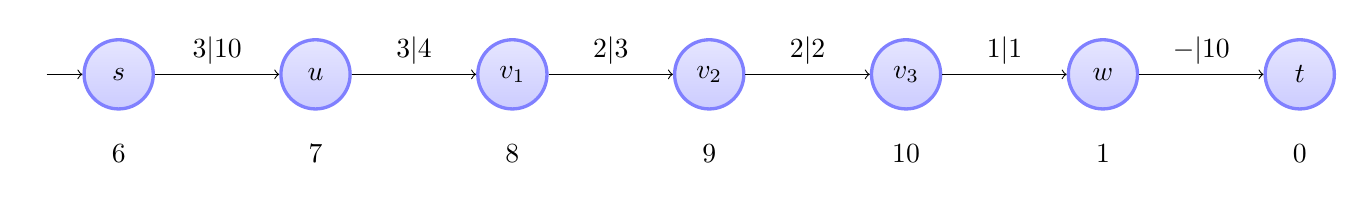
\begin{tikzpicture}[node distance=2.5cm,on grid,auto,bend angle=10]
	\tikzstyle{every state}=[very thick,fill=blue!20,draw=blue!50]
	\tikzstyle{every initial by arrow}=[initial text=]

	\node[state,initial,nodestyle]	(s)				{$s$};
		\node[below=1cm of s] {6};
	\node[state,nodestyle]			(u) [right=of s]  {$u$};
		\node[below=1cm of u] {7};
	\node[state,nodestyle]			(v1) [right=of u] {$v_1$};
		\node[below=1cm of v1] {8};
	\node[state,nodestyle]			(v2) [right=of v1] {$v_2$};
		\node[below=1cm of v2] {9};
	\node[state,nodestyle]			(v3) [right=of v2] {$v_3$};
		\node[below=1cm of v3] {10};
	\node[state,nodestyle]			(w) [right=of v3] {$w$};
		\node[below=1cm of w] {1};
	\node[state,nodestyle]			(t) [right=of w] {$t$};
		\node[below=1cm of t] {0};

\path[->] (s) edge node{$3|10$}(u)
			(u) edge node{$3|4$}(v1)
			(v1) edge node{$2|3$}(v2)
			(v2) edge node{$2|2$}(v3)
			(v3) edge node{$1|1$}(w)
			(w) edge node{$-|10$}(t);
\end{tikzpicture}
\[
	\text{new } Q = \{w,v_3,v_1\}
\]

\[
	\vdots
\]

After phase 8:\\
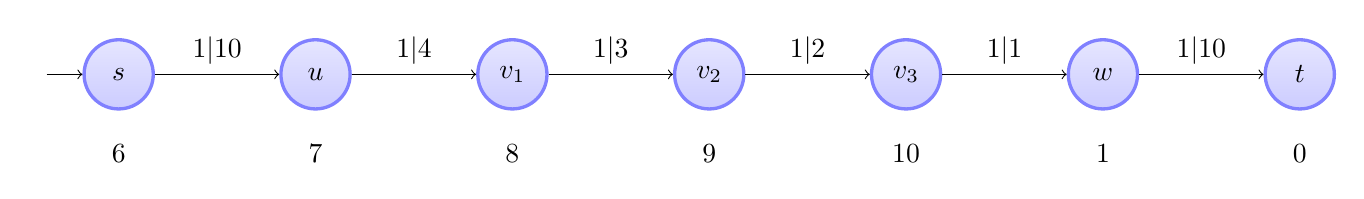
\begin{tikzpicture}[node distance=2.5cm,on grid,auto,bend angle=10]
	\tikzstyle{every state}=[very thick,fill=blue!20,draw=blue!50]
	\tikzstyle{every initial by arrow}=[initial text=]

	\node[state,initial,nodestyle]	(s)				{$s$};
		\node[below=1cm of s] {6};
	\node[state,nodestyle]			(u) [right=of s]  {$u$};
		\node[below=1cm of u] {7};
	\node[state,nodestyle]			(v1) [right=of u] {$v_1$};
		\node[below=1cm of v1] {8};
	\node[state,nodestyle]			(v2) [right=of v1] {$v_2$};
		\node[below=1cm of v2] {9};
	\node[state,nodestyle]			(v3) [right=of v2] {$v_3$};
		\node[below=1cm of v3] {10};
	\node[state,nodestyle]			(w) [right=of v3] {$w$};
		\node[below=1cm of w] {1};
	\node[state,nodestyle]			(t) [right=of w] {$t$};
		\node[below=1cm of t] {0};

\path[->] (s) edge node{$1|10$}(u)
			(u) edge node{$1|4$}(v1)
			(v1) edge node{$1|3$}(v2)
			(v2) edge node{$1|2$}(v3)
			(v3) edge node{$1|1$}(w)
			(w) edge node{$1|10$}(t);

\end{tikzpicture}
\[
	\text{new } Q = \emptyset
\]
\subsubsection*{b)}
\begin{center}
\begin{tabular}{r||c|c|c}
		\#pushes from node&	to the right & to the left & total\\\hline\hline
	$s$ & 0 & 0 & 0 \\\hline
	$u$ & 1 & 4 & 5 \\\hline
	$v_1$ & 1 & 3 & 4 \\\hline
	$v_2$ & 1 & 2 & 3 \\\hline
	$v_3$ & 1 & 1 & 2 \\\hline
	$w$ & 1 & 0 & 1 \\\hline
	$t$ & 0 & 0 & 0	
\end{tabular}\end{center}
\[
	\Ra \sum = 15
\]

\subsubsection*{c)}
\begin{center}
\begin{tabular}{r||c|c|c}
	\#pushes from node&	to the right & to the left & total\\\hline\hline
	$s$ & 0 & 0 & 0 \\\hline
	$u$ & 1 & k+1 & k+2 \\\hline
	$v_1$ & 1 & k & k+1 \\\hline
	$v_2$ & 1 & k-1 & k \\
	$\vdots$ &  &  &  \\\hline
	$v_{k-1}$ & 1 & 2 & 3 \\\hline
	$v$ & 1 & 1 & 2 \\\hline
	$w$ & 1 & 0 & 1 \\\hline
	$t$ & 0 & 0 & 0	
\end{tabular}\end{center}
\[
	\Ra \sum_{i=1}^{k+2} i = \frac{(k+2)(k+3)}{2}
\]

\subsection*{Task 3}
\begin{proof}
\begin{align*}
	\sum_{e\in E} f(e) \Delta(e) &= \sum_{(u,v) \in V^2} f(u,v) \cdot \Delta(u,v) = \sum_{(u,v)\in V^2} f(v,u) \cdot \bigl( \pi(v) - \pi(u) \bigr)\\
	&= \sum_{(u,v)\in V^2} f(u,v) \cdot \pi(v) - \sum_{(u,v)\in V^2} f(u,v) \cdot \pi(u)\\
	&= \sum_{v\in V} \pi(v) \cdot \sum_{u\in V} f(u,v) - \sum_{u\in V} \pi(u) \cdot \sum_{v\in V} f(u,v)\\
	&= \sum_{u\in V\setminus\{s,t\}} \pi(u)\cdot \sum_{v\in V} f(v,u) - \sum_{u\in V\setminus\{s,t\}} \pi(u) \cdot \sum_{v\in V} f(u,v)\\
	&\quad+ \pi(s) \underbrace{\sum_{v\in V} \bigl[ f(v,s) - f(s,v) \bigr]}_{-|f|} + \pi(t) \cdot \underbrace{\sum_{v\in V} \bigl[ f(v,t) - f(t,v) \bigr]}_{|f|} \quad (*)
\end{align*}
\end{proof}

\subsection*{Task 4}
\subsubsection*{a)}
Sketch: Double $y$ nodes; capacity 1 on every edge.

Construct a flow network $(G,s,t,c)$ as follows:
\[
	G=(V,Z) \text{ with}
\]\[
	V = \{s,t\} \cup X \cup Z \cup Y^{(1)} \cup Y^{(2)}
\]\[
	Y^{(i)} = \{y^{(i)} | y\in Y\}, i=1,2
\]\begin{align*}
	E&= \{ (s,x) | x\in X \} \cup \{ (x,y^{(1)})|(x,y)\in E_N \}\\
		&\quad \cup
		\{ (y_1^{(2)},y_2^{(1)}) | (y_1,y_2) \in E_N \}\\ 
		&\quad \cup \{ (y^{(2)},z) | (y,z) \in E_N \} \cup \{ (z,t) | z\in Z \}\\
		&\quad \cup	\{ (y^{(1)},y^{(2)}) | y\in Y \},\ c(e) = 1\ \forall e\in E
\end{align*}
\subsubsection*{b)}
$\ldots \Leftrightarrow (G,s,t,c)$ yields a flow $f$ with $|f| = |x|$
\subsubsection*{c)}
\textsc{MaxSucnFlow}, $\mathcal{O}(\sqrt{|V_N|} \cdot |E_N|)$

\end{document}